% =====================================================================================
%  Extract, Abstain, Generate -- NEXAI 2027 manuscript (Springer LNNS / llncs template)
%  Compile: pdflatex main -> bibtex main -> pdflatex main -> pdflatex main
%  Uses llncs.cls and splncs04.bst from the official NEXAI template (copies included).
%  All figures are vector graphics (TikZ / pgfplots), so resolution is unlimited.
% =====================================================================================
\documentclass[runningheads]{llncs}

\usepackage[T1]{fontenc}
\usepackage{amsmath,amssymb}
\usepackage{graphicx}
\usepackage{booktabs}
\usepackage{xcolor}
\usepackage{algorithm}
\usepackage{algorithmic}
\usepackage{tikz}
\usetikzlibrary{arrows.meta}
\usepackage{pgfplots}
\pgfplotsset{compat=1.17}
\usepackage[hidelinks]{hyperref}
\renewcommand\UrlFont{\color{black}\rmfamily}

\newcommand{\unk}{\textsc{unknown}}
\newcommand{\cond}[1]{\textsf{#1}}

% NEXAI 2027 review is double-blind: submit with \anonymoustrue (no names, affiliations,
% e-mails or identifying links). Switch to \anonymousfalse only for the camera-ready version.
\newif\ifanonymous
\anonymoustrue

\setlength{\textfloatsep}{6pt plus 2pt minus 2pt}
\setlength{\intextsep}{6pt plus 2pt minus 2pt}
\setlength{\floatsep}{6pt plus 2pt minus 2pt}
\renewcommand{\arraystretch}{0.93}
\setlength{\abovedisplayskip}{5pt plus 2pt minus 2pt}
\setlength{\belowdisplayskip}{5pt plus 2pt minus 2pt}
\setlength{\abovedisplayshortskip}{3pt plus 1pt minus 1pt}
\setlength{\belowdisplayshortskip}{3pt plus 1pt minus 1pt}

\linespread{0.985}
\begin{document}

\title{Extract, Abstain, Generate: Tracing Attribute Hallucination to Its Source in Image-Grounded Product Descriptions}
\titlerunning{Extract, Abstain, Generate}

\ifanonymous
\author{Anonymous Authors}
\authorrunning{Anonymous Authors}
\institute{Anonymous Institution}
\newcommand{\appname}{the deployed web application}
\else
\author{Vedanth C Y\thanks{Corresponding author.} \and Yashas B R \and Varun G Gowda \and Yashas H V \and Lokesh J K}
\authorrunning{V. C. Y. et al.}
\institute{School of Computer Science and Engineering, RV University, Bengaluru, Karnataka, India\\
\email{[e-mail of every author, in the order above]}}
\newcommand{\appname}{the TrueTag web application}
\fi

\maketitle

\begin{abstract}
Vision-language models are increasingly used to write e-commerce product descriptions, yet they often state product attributes that the image does not support. Grounding generation on attributes extracted by a separate classifier is a common remedy, but it leaves two questions open: when a grounded description is still wrong, which stage caused the error, and does an extractor's abstention survive the language model? This paper introduces an evaluation framework that attributes every category, color and material mention in a generated description to a vision-stage or a language-stage origin, using seven controlled conditions that include a gold-evidence oracle and a masked-attribute leakage probe. On a new benchmark of 240 double-annotated apparel images that includes Indian ethnic wear, two instruction-tuned language models of seven billion parameters add no attribute errors when given structured evidence: all hallucinations in the grounded pipeline originate in extraction.
Threshold-based abstention also survives the language stage (leakage of at most 0.5\% on extractor evidence) and removes material hallucination (0.58 to 0.00), although only because the extractor abstains on material for 98\% of items; category and color hallucination fall from 0.46 to 0.07 and from 0.45 to 0.15 relative to image-only models. A slot-based generator with a formal no-invention guarantee makes 70\% fewer unsupported claims per description but is rated far less fluent by human raters, whereas free-text generation with abstention is judged publishable as written for 93\% of descriptions. The labels and an offline, deployable system are released.
\keywords{Hallucination \and Vision-language models \and Selective prediction \and Abstention \and Grounded generation \and E-commerce \and Product descriptions}
\end{abstract}

% -------------------------------------------------------------------------------------
\section{Introduction}
Marketplaces need to catalog millions of items, and increasingly use visual-linguistic models (VLMs), like LLaVA~\cite{liu2023llava,liu2024llava15}, to produce descriptions of items based on product images. The models are competent, yet erroneous: They refer to a kurta as a dress, a navy colored shirt as a black one, or a plain t-shirt as ``100\% cotton.'' For instance, such attribute hallucinations come at an actual cost, because consumers rely on these exact attributes for filtering their search results.
One way to counter hallucinations is through \emph{grounding}: structure extraction with a dedicated classifier followed by writing with an LLM. Grounding transforms the question ``Does the model hallucinate?'' into two different and more concrete questions. One: When a grounded description is false, is the fault in the extraction process (vision stage) or in the writing process (language stage)? Two: If the extractor can produce \unk{} when it is unsure about its classification, does the writer maintain the uncertainty, or does he fill the void with a reasonable guess? Current benchmarks for model hallucination measure the output of a single model~\cite{rohrbach2018chair,li2023pope}.


\noindent\textbf{Research gap and objective.} Previous work checks whether the model is hallucinating but not at what stage in a two-stage process the hallucination occurs, and whether the abstention signal generated by one part of the model is adhered to by the next. The aim of this research is to track all the attribute errors in an image-based product description back to their origin stage and to check whether abstention flows through the language model, using an experimental setup where the only variation in the writing is the input from the writer.

\noindent\textbf{Contributions.}
\begin{itemize}\setlength{\itemsep}{0pt}\setlength{\topsep}{2pt}\setlength{\parsep}{0pt}
\item \textbf{Hallucination of attributes by stage classification}. Outcome and origin classification categorizes all attribute errors into extraction (extraction pass, EP) or writer error, generator deviation from truth (generator deviation, GD) or generator fabrication of an abstained attribute (generator fabrication, GF), using gold evidence as the oracle.
\item \textbf{Abstention-propagation evaluation metrics.} \emph{Leakage} and \emph{inflation} evaluate whether abstention propagates through the language model, in the thresholded output of the extractor and a gold-masked probe.
\item \textbf{Abstention-Preserving Generation (APG)}. Slot-and-render model that, compared to the claim extractor, never produces an attribute value except for the evidence, evaluated via free-text generation with automated and human metrics.
\item \textbf{A double-annotated benchmark} of 240 images of clothing (13 types like kurta and saree, 12 colors, 8 materials) with adjudicated annotations and human scores.
\item \textbf{Results and a working system.} Two LLM architectures do not introduce any attribute mistakes given structured information, and a pipeline of verification and correction designed based on this result can operate offline using a CPU.
\end{itemize}
As far as the authors know, this is the first paper to investigate the decomposition of attribute hallucinations in image-driven generation and study how abstention propagates within the language model.

\noindent \textbf{Motivation and outline of the paper.} The motivation is practical: a market place using grounded generation must decide whether to improve its classifier, its writing component or generation constraints, and an end-to-end hallucination rate cannot help there. The rest of the paper is structured as follows. Section~\ref{sec:related} provides background on the literature. Section~\ref{sec:method} provides details of the experimental conditions, the extractor with threshold abstention and the APG generator. Section~\ref{sec:eval} provides the evaluation framework and Section~\ref{sec:setup} the data and experimental setup. Results are reported in Section~\ref{sec:results}, which answers three research questions (RQ1 to RQ3). Deployment is discussed in Section~\ref{sec:discussion}. Limitations are listed in Section~\ref{sec:limits}.

% -------------------------------------------------------------------------------------
\section{Related Work}\label{sec:related}
\textbf{Hallucinations in vision-language models.} The CHAIR score~\cite{rohrbach2018chair} was introduced for counting objects mentioned in captions that are not present in the image; POPE~\cite{li2023pope} interrogates large vision-language models with yes/no questions, revealing that object hallucinations still occur even in instruction-tuned models like LLaVA~\cite{liu2023llava}. Surveys~\cite{ji2023survey} reveal hallucinations in generative models. AMBER~\cite{wang2023amber} tests attributes and relationships, FaithScore~\cite{jing2024faithscore} tests atomic statements within free-form responses, and visual contrastive decoding~\cite{leng2024vcd} prevents hallucinations within a single vision-language model. All of the above works test or fix a single model end-to-end, but this paper decomposes a two-stage pipeline and investigates which component made an error for each attribute.

\textbf{Attribute extractor faithfulness to structured input.} Data-to-text generation has long acknowledged the problem of neural generators expressing facts that do not appear in their input records~\cite{wiseman2017challenges} and has proposed table-aware metrics such as PARENT~\cite{dhingra2019parent}. Fact-level factuality metrics such as FActScore~\cite{min2023factscore} and LLM-as-a-judge evaluation~\cite{zheng2023judging} evaluate the truthfulness of individual supported and unsupported claims. The current approach incorporates a deterministic attribute checker and a LLM-based judge for non-attribute statements.

\textbf{Selective prediction.} Selective classifiers abstain when predictions' confidences fall below a certain threshold to favor accuracy over coverage~\cite{geifman2017selective}. Zero-shot dual encoders such as CLIP (Contrastive Language-Image Pre-training)~\cite{radford2021clip} and SigLIP (Sigmoid Loss for Language-Image Pre-training)~\cite{zhai2023siglip} offer scores that can be sufficiently calibrated to implement this concept into attribute extraction. Language model abstention has been thoroughly reviewed~\cite{wen2025abstention}, mostly because of properties of a single model's predictions. How such an abstention decision by one component is retained in the downstream generation process has not been evaluated in the surveyed literature.

\textbf{Generating product descriptions.} Online product description generation models make assumptions about the accuracy of the input attributes or the knowledge bases~\cite{chen2019kobe}. Product attribute values extraction based on textual information is a wide research domain where there exist MAVE~\cite{yang2022mave} dataset; however, in this study, the product attributes are extracted using images.
% -------------------------------------------------------------------------------------
\section{Methodology}\label{sec:method}

\subsection{Experimental Conditions}
For every product image, a description is produced under seven different experimental conditions (Fig.~\ref{fig:pipeline}): image generation alone with a generic prompt (\cond{A}), or a faithfulness prompt (\cond{A-F}); extraction followed by forced free-text writing using the extracted evidence (\cond{B}) or abstaining from writing based on extracted evidence (\cond{B-Abs}); extraction followed by slot writing with a renderer (\cond{APG}); and using gold labels as evidence: either complete evidence (\cond{C}) or partially hidden evidence (\cond{C-Mask}). Conditions \cond{B}, \cond{B-Abs}, \cond{C} and \cond{C-Mask} all employ the same prompt and just vary in the values of the evidence object $e=(e_{\text{cat}},e_{\text{col}},e_{\text{mat}})$.

\begin{figure}[!htb]
\centering
\resizebox{0.86\textwidth}{!}{%
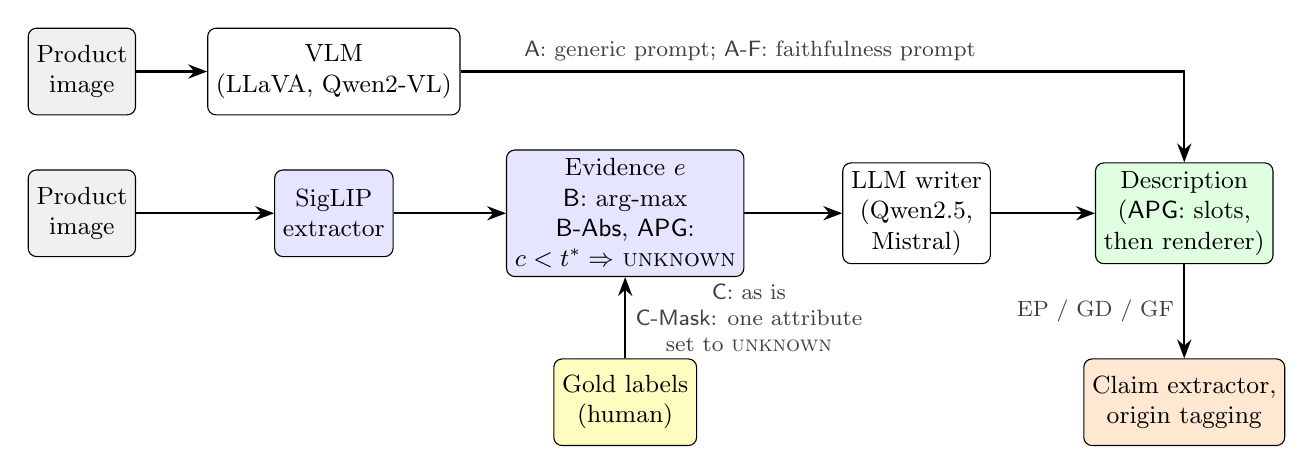
\begin{tikzpicture}[
  box/.style={draw, rounded corners=3pt, align=center, minimum height=1.1cm, inner sep=3pt, font=\small},
  img/.style={box, fill=gray!12},
  ext/.style={box, fill=blue!10},
  gold/.style={box, fill=yellow!25},
  outbox/.style={box, fill=green!12},
  arr/.style={-{Stealth[length=2.4mm]}, thick},
  lab/.style={font=\footnotesize, align=center, text=black!75}
]
\node[img] (ia) at (0,3.8) {Product\\image};
\node[box] (vlm) at (3.2,3.8) {VLM\\(LLaVA, Qwen2-VL)};
\draw[arr] (ia) -- (vlm);
\node[img] (ib) at (0,2) {Product\\image};
\node[ext] (ex) at (3.2,2) {SigLIP\\extractor};
\node[ext] (ev) at (6.9,2) {Evidence $e$\\\cond{B}: arg-max\\\cond{B-Abs}, \cond{APG}:\\$c<t^{*}\Rightarrow$ \unk};
\node[box] (wr) at (10.6,2) {LLM writer\\(Qwen2.5,\\Mistral)};
\draw[arr] (ib) -- (ex);
\draw[arr] (ex) -- (ev);
\draw[arr] (ev) -- (wr);
\node[gold] (gl) at (6.9,-0.4) {Gold labels\\(human)};
\draw[arr] (gl) -- node[right, lab] {\cond{C}: as is\\\cond{C-Mask}: one attribute\\set to \unk} (ev);
\node[outbox] (ds) at (14.0,2) {Description\\(\cond{APG}: slots,\\then renderer)};
\draw[arr] (wr) -- (ds);
\draw[arr] (vlm.east) -| node[above, pos=0.2, lab] {\cond{A}: generic prompt;\ \cond{A-F}: faithfulness prompt} (ds.north);
\node[box, fill=orange!18] (ce) at (14.0,-0.4) {Claim extractor,\\origin tagging};
\draw[arr] (ds) -- node[left, lab] {EP / GD / GF} (ce);
\end{tikzpicture}}
\caption{Pipeline and experimental conditions. The extractor's scores either pass as forced evidence (\cond{B}) or are thresholded into \unk{} (\cond{B-Abs}, \cond{APG}). Image-only baselines (\cond{A}, \cond{A-F}) bypass extraction; the oracle (\cond{C}) and the leakage probe (\cond{C-Mask}) replace extraction with human labels. Every hallucinated attribute is traced to its origin.}
\label{fig:pipeline}
\end{figure}

\subsection{Zero-Shot Extraction with Threshold-Driven Abstention}
For attribute $a$ with labels $\mathcal{L}_a$, each label has four prompt templates associated with it; their corresponding text embeddings are $\ell_2$ normalized, averaged, and re-normalized to obtain $\mathbf{t}_y$. For an image embedding $\mathbf{v}$, the label scores can be defined as $p(y\mid\mathbf{v})=\mathrm{softmax}_y(s\,\mathbf{v}^\top\mathbf{t}_y)$ using the logit scale $s$ from the model. The confidence score for attribute $a$ is $c_a=\max_y p(y\mid\mathbf{v})$. The forced evidence label is the arg-max label. The threshold is decided only on the development set by maximizing coverage under the constraint of selective accuracy $\tau$ (Equation \ref{eq:thresh}):
\begin{equation}
t_a^{*}=\min\{\,t : \mathrm{Acc}(\{i : c_{a,i}\geq t\})\geq\tau\,\},\qquad \tau=0.90.
\label{eq:thresh}
\end{equation}
The evidence $e_a=\unk$ is always assigned when $c_a < t_a^*$. Should no threshold ever meet $\tau$, the extractor will abstain from providing any value on $a$. Hence, Eq.~\ref{eq:thresh} balances coverage (percentage of items provided with a value) with the precision of those values.

\subsection{Abstention-Preserving Generation}
In APG, generation of attribute values is outside the writer's control. LLM is provided with placeholders \texttt{\{category\}}, \texttt{\{color\}} and \texttt{\{material\}} only for those attributes for which evidence is known, and is told to use placeholders in place of values. The output is post-processed using a deterministic renderer (Algorithm~\ref{alg:apg}).

\begin{algorithm}[!htb]
\footnotesize
\caption{APG renderer}
\label{alg:apg}
\begin{algorithmic}[1]
\REQUIRE LLM output $y$ with placeholders, evidence $e$
\STATE $S \leftarrow$ sentences of $y$
\STATE Remove $s\in S$ containing an invalid token, a stray brace, or a slot for an attribute with $e_a=\unk$
\STATE Fill remaining slots with $e_a$ and repair articles
\STATE Remove $s$ if the claim extractor finds in it any value $\neq e_a$, any mention of an abstained attribute, or a hedge
\IF{$S=\emptyset$ \OR the known category is not stated}
\STATE \textbf{return} template ``A \{color\} \{category\} in \{material\}.'' over known attributes
\ENDIF
\STATE \textbf{return} concatenation of $S$
\end{algorithmic}
\end{algorithm}

\begin{proposition}
For any evidence $e$ and any LLM output $y$, let $D_a(r)$ be the set of values of attribute $a$ claimed by the claim extractor for the rendered text $r$. Then $D_a(r)\subseteq\{e_a\}$ if $e_a$ is known, and $D_a(r)=\emptyset$ if $e_a=\mathrm{unknown}$.
\end{proposition}
\begin{proof}
Each sentence that survives line~4 of Algorithm~\ref{alg:apg} passes the verification step, which discards all sentences where the mentioned value deviates from $e$ or an abstained attribute is being mentioned; the fall-back template uses only known evidence values. Therefore, none of the returned sentences violate the property.
\end{proof}
This guarantee depends on the claim extractor (Section~\ref{sec:claims}) with the accuracy of 1.00 on the validation dataset. The guarantee was also validated against 25 hand-written adversarial LLM outputs.

% -------------------------------------------------------------------------------------
\section{Evaluation Framework}\label{sec:eval}
\subsection{Attribute Claim Extraction}\label{sec:claims}
An extractor based on deterministic lexicon matches each mention of category, color and material in a description using longest match priority ('t-shirt' never being interpreted as 'shirt'), proper word boundaries, plural and hyphen normalization, ignoring stylistic clauses ('pair it with blue jeans') and coloring of logos, prints and trims, and hedge detection. The category is always the first mention; the color and material are sets of values. It achieves precision 1.00 and recall 0.95-1.00 for attributes against labels agreed upon by two annotators (60 development descriptions).

\subsection{Outcomes and Origins}
The unit of analysis is a (description, attribute) pair with a gold label $g$, evidence $e$ (which is not available for \cond{A} and \cond{A-F}), and stated values $D$. A pair is \emph{correct} when $D=\{g\}$ for a gold label, a \emph{hallucination} when $D\neq\emptyset$ and $D\neq\{g\}$ (any value when $g=\unk$), an \emph{omission} when $D=\emptyset$ although a label was available, and a \emph{preserved abstention} when $D=\emptyset$ and $e=\unk$. Every hallucination with evidence gets exactly one origin, as defined in Eqs.~\ref{eq:ep}--\ref{eq:gf}:
\begin{align}
\text{EP}&: e\in\mathcal{L},\ D=\{e\},\ e\neq g \quad\text{(extraction passed)}\label{eq:ep}\\
\text{GD}&: e\in\mathcal{L},\ D\neq\{e\} \quad\text{(generator deviation)}\label{eq:gd}\\
\text{GF}&: e=\unk,\ D\neq\emptyset \quad\text{(generator fabrication)}\label{eq:gf}
\end{align}
EP (Eq.~\ref{eq:ep}) is a vision-stage error: The writer reproduced the wrong evidence. GD (Eq.~\ref{eq:gd}) and GF (Eq.~\ref{eq:gf}) are language-stage errors: the writer deviated from the right evidence, or filled attributes that were abstained from by the extractor. Since \cond{C} provides perfect evidence, the GD error rate for \cond{C} reflects only the writer's deviation; the origin test is a bootstrap confidence interval for $\mathrm{GD}(\cond{B}) - \mathrm{GD}(\cond{C})$.

\subsection{Abstention Propagation}
In pairs where there is evidence, leakage (Eq.~\ref{eq:leak}) is the percentage of abstained attributes that the writer still mentions, and inflation (Eq.~\ref{eq:infl}) is the percentage of non-abstained attributes that the writer omits or hedges:
\begin{align}
\mathrm{Leak}&=\frac{|\{e=\unk,\ D\neq\emptyset\}|}{|\{e=\unk\}|},\label{eq:leak}\\
\mathrm{Infl}&=\frac{|\{e\in\mathcal{L},\ D=\emptyset\ \lor\ \text{hedged}\}|}{|\{e\in\mathcal{L}\}|}.\label{eq:infl}
\end{align}
The low leakage indicates that abstinence is honored; the low inflation indicates that the author does not get too cautious. In \cond{C-Mask}, leakage is calculated for the masked attribute only, since the value is known and masked from the writer.

\subsection{Claims About Non-Attributes, Human Judgment and Statistics}
An LLM judge (Qwen2.5-7B) provides unsupported claims except for the attributes, category, color and material (fit, functionality, occasions, brand, etc.). The rate of unsupported claims (UCR) is the average number of unsupported claims per description. Since the judge tends to over-predict (precision 0.31, recall 0.68, compared to a human judge on 70 test descriptions), the absolute values of UCRs are upper estimates, although both agree that \cond{APG} has the lowest value. Descriptions from conditions \cond{A-F}, \cond{B-Abs} and \cond{APG} were rated by human judges for fluency, faithfulness and usefulness (1-5) and on whether they would be published as is, blinded to condition.

All rates include 95\% item-cluster bootstrap intervals (2,000 replications). Comparisons across all pairs are based on the exact McNemar test with Holm adjustment within each attribute and LLM; human ratings on the Wilcoxon signed-rank test; agreement measures Cohen's $\kappa$ and Krippendorff's $\alpha$.

% -------------------------------------------------------------------------------------
\section{Experimental Setup}\label{sec:setup}
\subsection{Data and Annotation}
Image dataset used is \emph{Fashion Product Images}~\cite{aggarwal2019fashion}. This is a 384$\times$512 resolution image (fabric clues being visible in higher resolution). After filtering 13 product categories with mappable colors (17,162 out of 44,072), seeded sampling results in 40 development images and 200 test images; 16\% of test images belong to ethnic wear (kurta and saree).

All images are annotated independently by two annotators. The category and color information are pre-filled from metadata and material information was left blank as it requires visual cue in images. There was only one guideline revision based on development images and the guidelines were frozen after that; the third annotator resolved all the disagreements. Test agreement (Cohen's $\kappa$) for category, color, and material is 1.00, 0.86, and 0.50 respectively. The low agreement of material can be attributed to its intrinsic difficulty; 15.5\% test images have gold material.

\subsection{Models and Configuration}
The extractors are CLIP ViT-L/14~\cite{radford2021clip} and SigLIP so400m~\cite{zhai2023siglip} (main model, due to lower AURC). The vision-language models are LLaVA-1.5-7B~\cite{liu2024llava15} (main) and Qwen2-VL-2B~\cite{wang2024qwen2vl}. The writers are Qwen2.5-7B-Instruct~\cite{yang2024qwen25} (main) and Mistral-7B-Instruct~\cite{jiang2023mistral}. All 7B parameters were trained using 4-bit NormalFloat (NF4)~\cite{dettmers2023qlora} on one 16 GB T4 GPU in greedy decoding. The prompts and thresholds were hashed and frozen prior to each test. Nothing was fine-tuned on the test dataset.

% -------------------------------------------------------------------------------------
\section{Results and Analysis}\label{sec:results}
\subsection{Extraction}
Table~\ref{tab:extraction} shows the performance of extraction on the test split. SigLIP beats CLIP on all attributes and orders its confidences better (smaller AURC), hence it is our main extractor. Zero-shot recognition of materials is close to random chance for both methods, therefore the development tuned decision rule causes SigLIP to abstain on materials for 98\% of items (CLIP always abstains). The selective accuracies of the two methods on test are 0.928 for categories and 0.827 for colors; the color figure is less than the 0.90 target, which means that the thresholds tuned using only 40 development items generalize poorly, and the difference is the reason for the 0.147 color hallucination rate shown below.

\begin{table}[!htb]
\caption{Extraction on the test split ($n=200$). Threshold $t^{*}$ is fixed on the development split; coverage and selective accuracy are evaluated at this threshold. CI: confidence interval; AURC: area under the risk-coverage curve; Sel.\ acc.: selective accuracy.}
\label{tab:extraction}
\centering
\footnotesize
\setlength{\tabcolsep}{3.5pt}
\begin{tabular}{@{}llcccccc@{}}
\toprule
Extractor & Attribute & Forced acc.\ [95\% CI] & AURC & $t^{*}$ & Coverage & Sel.\ acc. \\
\midrule
CLIP ViT-L/14 & category & 0.845 [0.790, 0.895] & 0.050 & 0.566 & 91.5\% & 0.869 \\
 & color & 0.658 [0.587, 0.728] & 0.144 & 0.914 & 29.9\% & 0.945 \\
 & material & 0.491 [0.414, 0.568] & 0.539 & n/a$^{\dagger}$ & 0\% & -- \\
\midrule
SigLIP so400m & category & 0.910 [0.870, 0.950] & 0.022 & 0.501 & 97.0\% & 0.928 \\
 & color & 0.772 [0.707, 0.832] & 0.092 & 0.605 & 84.8\% & 0.827 \\
 & material & 0.497 [0.420, 0.574] & 0.478 & 0.986 & 2.0\% & 1.000 \\
\bottomrule
\end{tabular}

\smallskip
\footnotesize $^{\dagger}$No threshold attains the 0.90 target, so the extractor always abstains.
\end{table}

\subsection{Main Results}
Results on hallucination rates are given in Table~\ref{tab:main} and Fig.~\ref{fig:hr}. Image-only VLM hallucinate about the category or color of the object about half the time, and a faithfulness prompt does not help except for the color of the object (the effect is significant, Holm-adjusted $p=0.034$). Grounding decreases hallucinations of the category from 0.46 (\cond{A-F}) to 0.07, and of color from 0.45 to 0.15 with the abstention mechanism (exact McNemar test, Holm-adjusted $p=1.3\times10^{-18}$ and $3.7\times10^{-13}$). Forced grounding (\cond{B}) describes material for each object and makes mistakes in 58\% cases; abstention eliminates all 116 mistakes ($p=1.2\times10^{-34}$), and also reduces color hallucination rate from 0.228 to 0.147 ($p=1.8\times10^{-4}$). Zero material hallucination rates of VLM mean silence rather than correctness of predictions: LLaVA describes material in 0.5\% of the descriptions.

\begin{table}[!htb]
\caption{Hallucination rate on the test split (primary configuration), with 95\% bootstrap intervals. \cond{C-Mask} reports hallucination (a wrong value), which is smaller than its leakage (Table~\ref{tab:abst}) since a leaked value may be true.}
\label{tab:main}
\centering
\footnotesize
\setlength{\tabcolsep}{4pt}
\begin{tabular}{@{}lccc@{}}
\toprule
Condition & Category & Color & Material \\
\midrule
\cond{A} & .445 {\scriptsize[.375,.515]} & .516 {\scriptsize[.446,.592]} & .000 \\
\cond{A-F} & .460 {\scriptsize[.390,.530]} & .451 {\scriptsize[.375,.527]} & .000 \\
\cond{B} & .090 {\scriptsize[.050,.130]} & .228 {\scriptsize[.168,.293]} & .580 {\scriptsize[.515,.650]} \\
\cond{B-Abs} & \textbf{.070} {\scriptsize[.035,.110]} & \textbf{.147} {\scriptsize[.103,.201]} & \textbf{.000} \\
\cond{APG} & \textbf{.070} {\scriptsize[.035,.110]} & \textbf{.147} {\scriptsize[.103,.201]} & \textbf{.000} \\
\cond{C} & .000 & .000 & .000 \\
\cond{C-Mask} & .009 {\scriptsize[.002,.018]} & .000 & .000 \\
\bottomrule
\end{tabular}
\end{table}

\begin{figure}[!htb]
\centering
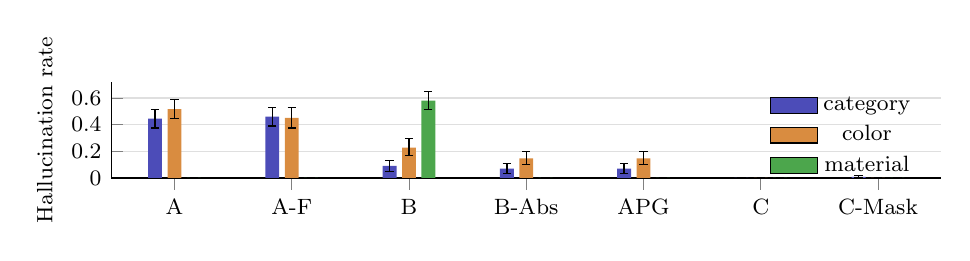
\begin{tikzpicture}
\begin{axis}[
  ybar, bar width=5pt, width=\textwidth, height=2.8cm, area legend, axis x line*=bottom, axis y line*=left,
  symbolic x coords={A,A-F,B,B-Abs,APG,C,C-Mask}, xtick=data,
  ymin=0, ymax=0.72, ylabel={Hallucination rate},
  ymajorgrids, grid style={gray!25},
  legend style={at={(0.98,0.97)}, anchor=north east, font=\footnotesize, draw=none, fill=none},
  tick label style={font=\footnotesize}, label style={font=\footnotesize},
  enlarge x limits=0.09,
  error bars/y dir=both, error bars/y explicit,
  error bars/error bar style={black, line width=0.5pt},
  error bars/error mark options={rotate=90, mark size=1.5pt, black}
]
\addplot[fill=blue!60!black!70, draw=none] table[x=c, y=v, y error plus=p, y error minus=m, row sep=\\] {
c v p m \\
A .445 .070 .070 \\
A-F .460 .070 .070 \\
B .090 .040 .040 \\
B-Abs .070 .040 .035 \\
APG .070 .040 .035 \\
C .000 0 0 \\
C-Mask .009 .009 .007 \\
};
\addplot[fill=orange!80!black!75, draw=none] table[x=c, y=v, y error plus=p, y error minus=m, row sep=\\] {
c v p m \\
A .516 .076 .070 \\
A-F .451 .076 .076 \\
B .228 .065 .060 \\
B-Abs .147 .054 .044 \\
APG .147 .054 .044 \\
C .000 0 0 \\
C-Mask .000 0 0 \\
};
\addplot[fill=green!50!black!70, draw=none] table[x=c, y=v, y error plus=p, y error minus=m, row sep=\\] {
c v p m \\
A .000 0 0 \\
A-F .000 0 0 \\
B .580 .070 .065 \\
B-Abs .000 0 0 \\
APG .000 0 0 \\
C .000 0 0 \\
C-Mask .000 0 0 \\
};
\legend{category, color, material}
\end{axis}
\end{tikzpicture}
\caption{Hallucination rate by condition and attribute (test split, $n=200$; whiskers: 95\% bootstrap intervals).}
\label{fig:hr}
\end{figure}

\subsection{RQ1: Where Do Grounded Hallucinations Arise?}
In \cond{B}, all hallucinations arise from extraction errors; the EP rates of category, color and material are 0.09, 0.23 and 0.58, and GD and GF are 0.00 for Qwen2.5 in all attributes, which amounts to an extraction ratio of 1.00. Mistral has only one GD error (with a rate of 0.005) in 387 hallucinations, resulting in an extraction ratio of 0.991. Origin analysis shows that there is no deviation added by the writer to the oracle: $\mathrm{GD}(\cond{B})-\mathrm{GD}(\cond{C})=0.000$ [0.000, 0.000] for Qwen2.5 and at most 0.005 [0.000, 0.015] for Mistral. The two groups of LLMs agree in 99.3\% of all pair-based cases, therefore structured evidence means the writer is a faithful copier.

\subsection{RQ2: Is Abstention Robust to the Language Model?}
Yes (Table~\ref{tab:abst}). For Qwen2.5, both \cond{B-Abs} and \cond{APG} have no leakage and inflation for each attribute; Mistral is prone to leaking at most 0.005 and dropping at least one known category (inflation 0.031). The only significant leakage occurs for \cond{C-Mask}: despite having a masked category, Qwen2.5 still labels a garment in 5\% of the descriptions, and all ten of those leaks label ``jeans'', inferred from ``denim'' in the rest of the evidence.

\begin{table}[!htb]
\caption{Abstention propagation: leakage and inflation (SigLIP evidence); the attribute with the maximum value is in parentheses.}
\label{tab:abst}
\centering
\footnotesize
\setlength{\tabcolsep}{5pt}
\begin{tabular}{@{}llcc@{}}
\toprule
Condition & Writer & Leakage (max) & Inflation (max) \\
\midrule
\cond{B-Abs} & Qwen2.5 & 0.000 & 0.000 \\
\cond{B-Abs} & Mistral & 0.005 (material) & 0.031 (category) \\
\cond{APG} & Qwen2.5 & 0.000 & 0.000 \\
\cond{APG} & Mistral & 0.000 & 0.026 (color) \\
\cond{C-Mask} & Qwen2.5 & 0.050 (category) & 0.000 \\
\cond{C-Mask} & Mistral & 0.020 (category) & 0.045 (category) \\
\bottomrule
\end{tabular}
\end{table}

\subsection{RQ3: Is APG Beneficial without Compromising Quality?}
APG is equivalent to \cond{B-Abs} in terms of attribute hallucination (both get the same evidence and both copy it) while decreasing unsupported non-attribute statements from 0.57 to 0.17 per description, which is a decrease of 70\%, not taking into account the description length (Table~\ref{tab:human}, see Section~\ref{sec:limits}), and its template renderer was used by 6\% of the items with Qwen2.5 and 2\% of the items with Mistral. Yet, humans greatly favor free-text descriptions: \cond{B-Abs} gets 4.30, 4.37 and 4.15 points for fluency, faithfulness and usefulness, respectively, compared to 1.67, 2.17 and 1.72 points for APG (Wilcoxon, Holm $p<10^{-4}$ on all scales) with 93\% of \cond{B-Abs} descriptions publishable ``as is''. The brief, templated descriptions generated by APG score lower even in terms of faithfulness than the erroneous \cond{A-F} baseline ($p=0.012$). Krippendorff's $\alpha$ is 0.88 and 0.81 for fluency and usefulness, respectively, and 0.57 for faithfulness.

\begin{table}[!htb]
\caption{Unsupported non-attribute claims (UCR) and human evaluation (30 items, mean of 2 raters, 95\% bootstrap interval). ``Publish'' is the share of descriptions that raters would publish as written.}
\label{tab:human}
\centering
\footnotesize
\setlength{\tabcolsep}{3pt}
\begin{tabular}{@{}lcccccc@{}}
\toprule
Condition & UCR & Fluency & Faithfulness & Usefulness & Publish \\
\midrule
\cond{A-F} & 1.02 & 2.15 [1.97, 2.33] & 3.03 [2.77, 3.28] & 2.12 [1.88, 2.37] & 0.08 \\
\cond{APG} & \textbf{0.17} & 1.67 [1.30, 2.10] & 2.17 [1.77, 2.58] & 1.72 [1.38, 2.07] & 0.23 \\
\cond{B-Abs} & 0.57 & \textbf{4.30} [4.07, 4.52] & \textbf{4.37} [4.20, 4.53] & \textbf{4.15} [3.90, 4.38] & \textbf{0.93} \\
\bottomrule
\end{tabular}
\end{table}

\subsection{Local Wear}
Category hallucination by image-only VLMs is highest for ethnic clothes: 0.75 (\cond{A}) and 0.88 (\cond{A-F}) for kurtas and sarees (32 images) compared to 0.39 and 0.38 for western clothes (168 images); also, out of the 24 category mistakes made by LLaVA on the former type, 22 classify them as dresses. Category classification of SigLIP is perfect (1.000 vs 0.893 for western clothes), thus grounding significantly reduces the gap (\cond{B-Abs} category classification rate of 0.03 vs 0.11), although multicolor ethnic clothes still pose more challenges in terms of color (\cond{B-Abs} color rate of 0.16 vs 0.07).

% -------------------------------------------------------------------------------------
\section{Discussion and Deployment}\label{sec:discussion}
\textbf{Fix perception, not the writer.} With structured data, instructions-tuned 7 billion parameter writers do not wander away from or create attributes; therefore, faithful generation of attributes is limited to the extractor. It is more productive to focus efforts on refining perception.

\textbf{Abstinence is inexpensive but costly for coverage.} Thresholds tuned to 40 labeled items identified all material errors on test data and transferred to two writer families, but materials are seldom mentioned because zero-shot extractors cannot read fabric from catalogue photos.

\textbf{Guarantees vs. readability.} Hard guarantees seem to strip out all unfounded free-text statements (70\% reduction per description, depending on the limitations of Section~\ref{sec:limits}) but yield descriptions that people do not want to read. Free-text generation with abstention, verification, and repair is thus advocated because it maintains the attribute guarantee only when necessary. This scheme is realized in \appname, which is SigLIP extraction with the fixed thresholds, a 1.5 billion parameter writer, and the claim extractor as the verifier repairing draft descriptions of unsupported attributes using APG. The algorithm runs offline on a laptop CPU with 16\,GB RAM, taking 20\,s per image.

% -------------------------------------------------------------------------------------
\section{Limitations}\label{sec:limits}
The benchmark is tiny (200 test items, one product domain and dataset), therefore estimates of each category have large confidence intervals. Material agreement ($\kappa=0.50$) is lower than the standard 0.6 threshold, and category and color labels were checked from pre-filled metadata, which may bias towards conventions used in metadata. The human experiment involved 30 items and two raters, and the judge was calibrated with the single labeler. Models were quantized to 4-bits and greedy decoded with a single prompt; larger or unquantized models could differ. The APG guarantee applies only to the lexicon-based claim extractor, which evaluates attribute hallucination, hence equal rates of APG and \cond{B-Abs} are mostly designed in. The 70\% reduction in unsupported non-attribute claims is not adjusted to description length, and APG responses are brief by design, therefore some part of it is due to shorter descriptions; the judge over-counts (precision 0.31) and was calibrated with the single labeler. Abstention is not fully calibrated: color selective accuracy on test (0.827) was below the 0.90 target, and the reduction of material errors is due to the coverage loss (98\% abstention).

% -------------------------------------------------------------------------------------
\section{Conclusion}\label{sec:conclusion}
The study pinpointed the source of the attribute hallucination phenomenon in image-grounded product descriptions. The use of structured evidence ensures that there are no errors introduced by the language models when hallucinating attributes (generator deviation is at most 0.005 [0.000, 0.015]). The threshold abstention approach not only persists but performs flawlessly in the generation stage (leakage is at most 0.005 based on the extractor’s evidence) and filters out all 116 material errors ($p=1.2 \times 10^{-34}$), but at the expense of mentioning material in only 2\% of items. Image grounding coupled with abstention filters out category and color hallucination from 0.46 to 0.07 and 0.45 to 0.15 compared to the image-only model ($p < 10^{-12}$) while the generated text is acceptable for publishing as is in 93\% of the descriptions while a no invention constraint is less fluent.

\subsubsection*{Data and Code Availability.}
\ifanonymous
Code, item identifiers, labels and the application will be released publicly upon acceptance.
\else
Code, item identifiers, labels and the application are available at \url{https://github.com/Yashas-BR/grounded-product-description} and \url{https://github.com/Yashas-BR/TrueTag_Product_Description}.
\fi

\bibliographystyle{splncs04}
\bibliography{references}

\end{document}
